\section{Results - Elicitation of parameters}
\label{ResultsElicitation}
%
%I må gerne tjekke oversættelsen på SQ og labels, så sletter vi de danske SQ efterfølgende og skriver det vigtige
%
Based on the 10 categories a variable can be elicited according to the criterion of a) being an influencing variable and b) the possibility of formulating the variable as a scale question. The field study was conducted on Danish speaking test subjects, and thus the variables are listed in both English and Danish. The scale questions are all presented on a \textit{Visual Analoge Scale} (VAS) with closed anchor points and are either bi- or unipolar. If the scale is bipolar a mid point will be marked either with or without a label. A bipolar scale without a label will be noted with \textit{No label}, whereas an unipolar scale which does not contain a mid point will be noted with a \textit{-}. 

In the following the 23 derived scales (noted \textit{S}), along with the specific scale question (noted \textit{SQ}), will be presented in corresponding order as presented for the test subjects in Experiment 2 and not according to the specific categories.\\ 

\noindent
SQ1: How do think the screen on the robot reacted? (Hvordan synes du, at skærmen på robotten reagerede?)\\
SQ2: How did you experience the robot? (Hvordan oplevede du robotten?)\\
SQ3: How was it to use the robot? (Hvordan var det at bruge robotten?)\\
SQ4: How did you experience the robots movements? (Hvordan oplevede du robottens bevægelser?)\\
For each of the four scale questions the chosen labels are listed in \autoref{tab:ScalesPage1}.
%
\begin{table}[H]
	\centering
\caption{Scale labels PAGE 1}
	\label{tab:ScalesPage1} 
	\begin{tabular}{l|c|c|c}
		S     & Left label & Mid point & Right label \\\hline
		1   & \makecell{Extremely bad\\(Ekstremt dårligt)}  & No label & \makecell{Extremely well \\(Ekstremt godt)}        \\\hline
		2   & \makecell{Extremely unwelcoming \\(Ekstremt afvisende)} & No label & \makecell{Extremely welcoming \\(Ekstremt imødekommende)}         \\\hline
		3   & \makecell{Extremely difficult \\(Ekstremt svært)} & No label & \makecell{Extremely easy \\(Ekstremt nemt)}         \\\hline
	 	4   & \makecell{Extremely wild \\(Ekstremt vilde)} & No label & \makecell{Extremely calm \\(Ekstremt rolige)}               
	\end{tabular}        
\end{table}
\noindent
%
Each of the four scale questions mentioned above will be presented on scales similar to the one shown on \autoref{fig:TilpassetSkaermensReaktion}, which corresponds to SQ1. The remaining three SQs will be presented on the same type of scale with their corresponding labels listed in \autoref{tab:ScalesPage1}.  
%
\begin{figure}[H]
\centering

\includegraphics[width = 0.49\textwidth]{Figure/TilpassetSkaermensReaktion}
\setlength\abovecaptionskip{-1.2\baselineskip} 
\caption{Example of an bipolar scale relevant for the scale question: \textit{How do think the screen on the robot reacted?}.}
\label{fig:TilpassetSkaermensReaktion}
\end{figure}
\noindent
% 
SQ5: I think that the robot stopped... (Jeg synes, at robotten stoppede...)\\
SQ6: I think that the robot's speed is... (Jeg synes, at robottens hastighed er...)\\ 
SQ7: I think that the robot's height is... (Jeg synes, at robottens højde er..)\\
For each of the three scale questions the chosen labels are listed in \autoref{tab:ScalesPage2}.  
%
\begin{table}[H]
	\centering
\caption{Scale labels PAGE 2}
	\label{tab:ScalesPage2} 
	\begin{tabular}{l|c|c|c}
		S     & Left label & Mid point & Right label \\\hline
		5   & \makecell{Way too close\\(Alt for tæt på)}  & No label & \makecell{Way too far \\(Alt for langt fra)}        \\\hline
		6   & \makecell{Way too slow\\(Alt for langsom)} & \makecell{Fine\\(Fin)} & \makecell{Way too fast \\(Alt for hurtig)}         \\\hline
		7   & \makecell{Way too low \\(Alt for lav)} & \makecell{Fine\\(Fin)} & \makecell{Way too high\\(Alt for høj)}                
	\end{tabular}        
\end{table}
\noindent
%
Each of the three scale questions mentioned above will be presented on scales similar to the one shown on \autoref{fig:TilpassetRStoppede}, which corresponds to SQ5. The remaining two SQs will be presented on the same type of scale with their corresponding labels and mid points listed in \autoref{tab:ScalesPage2}.  
%
\begin{figure}[H]
\centering
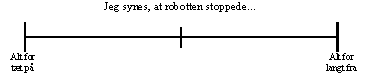
\includegraphics[width = 0.49\textwidth]{Figure/TilpassetRStoppede}
\setlength\abovecaptionskip{-1.2\baselineskip} 
\caption{Example of an bipolar scale relevant for the scale question: \textit{I think that the robot stopped...}}
\label{fig:TilpassetRStoppede}
\end{figure}
\noindent
% 
SQ8: I feel that the robot can help me (Jeg føler, at robotten kan hjælpe mig)\\
SQ9: I think that the robot was obstructing (Jeg synes, at robotten stod i vejen)\\
SQ10: I feel safe around the robot (Jeg føler mig tryg ved robotten)\\
SQ11: The robot startled me (Robotten gjorde mig forskrækket)\\
SQ12: I like to be served by the robot (Jeg kan godt lide at blive betjent af robotten)\\
SQ13: I counted on the robot to lead me to the location I chose (Jeg regnede med, at robotten fulgte mig hen til det sted jeg valgte)\\
Each of the six scale questions will be presented on the same type of scale with the same labels, as listed in \autoref{tab:ScalesPage3}. However, when presented for the subjects in Experiment 2 the scales will be presented three and three in the same order as presented above.   
%
\begin{table}[H]
	\centering
\caption{Scale labels for SQ8 to SQ13}
	\label{tab:ScalesPage3} 
	\begin{tabular}{l|c|c|c}
		S     & Left label & Mid point & Right label \\\hline
		8-13   & \makecell{Completely disagree\\(Helt uenig)}  & No label & \makecell{Completely agree\\(Helt enig)}                      
	\end{tabular}        
\end{table}
\noindent
%
The six aforementioned scales will be presented on scales similar to the one shown on \autoref{fig:TilpassetRobottenKanHjaelpe}, with their corresponding scale questions. 
%
\begin{figure}[H]
\centering
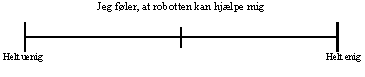
\includegraphics[width = 0.49\textwidth]{Figure/TilpassetRobottenKanHjaelpe}
\setlength\abovecaptionskip{-1.9\baselineskip} 
\caption{Example of an bipolar scale relevant for the scale question: \textit{I feel that the robot can help me}.}
\label{fig:TilpassetRobottenKanHjaelpe}
\end{figure}
\noindent
% 
SQ14: How personal did you experience the robot's help? (Hvor personlig oplevede du robottens hjælp?)\\
SQ15: How surprised were you when the robot made contact? (Hvor overrasket blev du over robottens henvendelse?)\\
For each of the two scale questions the chosen labels are listed in \autoref{tab:ScalesPage5}. 
%
\begin{table}[H]
	\centering
\caption{Scale labels PAGE 5}
	\label{tab:ScalesPage5} 
	\begin{tabular}{l|c|c|c}
		S     & Left label & Mid point & Right label \\\hline
		14   & \makecell{Not at all personal\\(Slet ikke personlig)}  & - & \makecell{Extremely personal\\(Ekstremt personlig)}        \\\hline
		15   & \makecell{Not at all surprised\\(Slet ikke overrasket)} & - & \makecell{Extremely surprised \\(Ekstremt overrasket)}               
	\end{tabular}        
\end{table}
\noindent
%
The two scales listed in \autoref{tab:ScalesPage5} will be presented on an unipolar scale with corresponding labels. \autoref{fig:TilpassetPersonligHjaelp} shows the scale for SQ14. 
%
\begin{figure}[H]
\centering
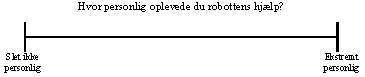
\includegraphics[width = 0.49\textwidth]{Figure/TilpassetPersonligHjaelp}
\setlength\abovecaptionskip{-1.2\baselineskip} 
\caption{Example of an bipolar scale relevant for the scale question: \textit{How personal did you experience the robots help?}.}
\label{fig:TilpassetPersonligHjaelp}
\end{figure}
\noindent
% 
The following eight scales, presented with two different scale questions, will also be presented on scales similar to the one shown on \autoref{fig:TilpassetPersonligHjaelp}, with their own labels. \\  
SQ16: What do you think about the robot? (Hvad synes du om robotten)\\
This scale question covers four different scales on which different parametres can be evaluated, these scales are presented with corresponding labels in \autoref{tab:ScalesPage6}. 
%
\begin{table}[H]
	\centering
\caption{Scale labels PAGE 6}
	\label{tab:ScalesPage6} 
	\begin{tabular}{l|c|c|c}
		S     & Left label & Mid point & Right label \\\hline
		16   & \makecell{Not at all annoying\\(Slet ikke irriterende)}  & - & \makecell{Extremely annoying \\(Ekstremt irriterende)}        \\\hline
		17   & \makecell{Not at all elegant \\(Slet ikke elegant)} & - & \makecell{Extremely elegant \\(Ekstremt elegant)}         \\\hline
		18   & \makecell{Not at all exciting\\(Slet ikke spændende)} & - & \makecell{Extremely exciting \\(Ekstremt spændende)}         \\\hline
	 	19   & \makecell{Not at all sweet \\(Slet ikke sød)} & - & \makecell{Extremely sweet \\(Ekstremt sød)}               
	\end{tabular}        
\end{table}
\noindent
%
SQ17: What else do you think about the robot? (Hvad synes du ellers om robotten?)\\
As with the aforementioned scale question, this scale question covers four different scales on which different parametres can be evaluated, these scales are presented with corresponding labels in \autoref{tab:ScalesPage7}  
%
\begin{table}[H]
	\centering
\caption{Scale labels PAGE 7}
	\label{tab:ScalesPage7} 
	\begin{tabular}{l|c|c|c}
		S    & Left label & Mid point & Right label \\\hline
		1   & \makecell{Not at all cool\\(Slet ikke sej)}  & - & \makecell{Extremely cool \\(Ekstremt sej)}        \\\hline
		2   & \makecell{Not at all intrusive \\(Slet ikke anmassende)} & - & \makecell{Extremely intrusive \\(Ekstremt anmassende)}         \\\hline
		3   & \makecell{Not at all funny\\(Slet ikke sjov)} & - & \makecell{Extremely funny \\(Ekstremt fun)}         \\\hline
	 	4   & \makecell{Not at all human \\(Slet ikke menneskelig)} & - & \makecell{Extremely human \\(Ekstremt menneskelig)}               
	\end{tabular}        
\end{table}
\noindent
%
Based on the affinity diagram a 24th parameter was derived, this parameter will not be presented along side the aforementioned scales but will be included in a seperat demographic page as it does not concern the robot. The parameter is formulated in the scale question: \textit{How happy are you with technology?}, which will be evaluated on a unipolar scale, similar to all other unipolar scales, with anchor points: \textit{Not at all happy} (slet ikke glad) and \textit{Extremely happy} (ekstremt glad).\\  

\noindent
When comparing the variables for HRI found in this study with variables for HRI from previous conducted studies on social robots \cite{PDF:ExploringInfluencingVariable}, \cite{PDF:SharingALifeHarvey}, \cite{PDF:InTheCompanyofRobots}, \cite{PDF:CloseButNotStuck}, \cite{PDF:TheImpactOfTraveler}, \cite{PDF:HumanRobotEmodiedInteraction}, \cite{PDF:RecommendationEffects}, variables such as distance, anthropomorphism, height, speed, movement, trust, enjoyment, technological knowledge, and usefulness reoccur. New variables, which probably are measured indirectly in the aforementioned variables, were found compared with previous mentioned studies these are: Elegance, sweet, cool, startled, exciting, welcoming, obstructive, robot help as personal, and wether the encounter with the robot was surprising. 

Accordring to \cite{PDF:HowSocialDistanceShapesHRI} \textit{social distance} has an effect on HRI, and even though the subjects did not mention it specifically. It seems that this is due to \textit{power distance}, where the subjects feel in control as they were the dominant part and the robot was the subordinate in the interaction. Furthermore this could also be do to the given task, the HRI, being cooperative as the robots purpose was to help the subject to a specific location of their choosing. When focusing on \textit{task distance} when in cooperative tasks it seems as if the subjects acted more friendly, intimate, and involved in the interaction with the robot, which is based on all the positive comments from subjects.       
 
  




